% Sports Engineering submission candidate
% Springer Nature template version 3.1 (December 2024)
\documentclass[lineno,pdflatex,sn-mathphys-num]{sn-jnl}

\usepackage{graphicx}
\usepackage{amsmath,amssymb}
\usepackage{booktabs}
\usepackage{multirow}
\usepackage{tikz}
\usetikzlibrary{arrows.meta,positioning,fit}

\definecolor{viewblue}{HTML}{0072B2}
\definecolor{vieworange}{HTML}{D55E00}
\definecolor{fusiongreen}{HTML}{009E73}
\definecolor{neutralgray}{HTML}{666666}

\raggedbottom

\begin{document}

\title[Evaluating two-view 3D pose fusion]
{Evaluating calibration-free two-view 3D pose fusion for exploratory repeated-cycle gymnastics analysis}

\author*[1]{\fnm{Kaixu} \sur{Chen}}\email{chenkaixusan@gmail.com}
\affil*[1]{\orgname{CCS}}

\abstract{Markerless three-dimensional motion analysis from ordinary video is
attractive for sports settings, but monocular estimates remain dependent on
camera view, occlusion and depth ambiguity. We evaluated how reliably two
temporally aligned monocular pose streams can be reused when camera calibration
and independent three-dimensional labels are unavailable. Face- and side-view
poses were transformed to a pelvis-centred body frame, after which a
view-order-invariant temporal network predicted a bounded correction using
rotation, skeletal and temporal self-supervision. In 137 participants
performing a repeated gymnastics movement, body-frame averaging reduced mean
distance to a same-video triangulated pseudo-reference by 47.54\% relative to
world-coordinate averaging; several aligned deterministic variants performed
similarly. On 14 held-out participants, the complete learned model reached
60.78~mm mean per-joint position error after sequence-level similarity
alignment and was statistically indistinguishable from arithmetic averaging
(60.85~mm) and the preceding learned ablation (60.80~mm). External testing on
199 Unity samples showed no zero-shot advantage over direct three-dimensional
averaging (178.506 versus 166.537~mm), whereas calibrated two-dimensional
triangulation reached 30.259~mm. Person-disjoint inference yielded 928 cycles
from 80 elderly-labeled and 57 student-labeled participants. Cohort contrasts
in angular speed and dimensionless jerk changed materially with the pose
source. Coordinate canonicalization, rather than the learned correction,
provided the clearest in-domain engineering gain. The resulting representation
supports exploratory sequence analysis, not absolute biomechanical measurement
or causal conclusions about ageing.}

\keywords{markerless motion capture, self-supervised learning, data fusion,
human movement, trunk rotation, repeated measures}

\maketitle

\noindent\textbf{Article counts:} approximately 2,500 words in the main body; 2
figures; 3 tables. Online Resource 1 contains 6 supplementary tables.

\section{Introduction}\label{sec:introduction}

Three-dimensional (3D) motion analysis can support technique assessment,
screening and feedback in sport, but laboratory motion capture is not always
available where movements are practised. Video-based systems lower the capture
burden. Modern monocular estimators can recover a dense articulated body from
one ordinary camera; SAM 3D Body, for example, predicts a full-body mesh and
Momentum Human Rig skeleton from an image \cite{Yang2026SAM3DBody}. A monocular
3D estimate nevertheless inherits depth ambiguity, self-occlusion, motion blur,
truncation and uncertain scale. Face and side cameras observe different
failures, so two predicted pose streams are potentially complementary but
cannot be averaged safely in their original coordinates.

Most multi-view methods combine images or two-dimensional (2D) evidence using
known or estimated camera geometry \cite{Iskakov2019Learnable,Qiu2019CrossView,
Remelli2020Lightweight,Jiang2023Probabilistic}. Other self-supervised approaches
learn from multi-view consistency but still begin from images or 2D poses
\cite{Kim2022CrossViewSelfFusion,Usman2022MetaPose,Srivastav2024SelfPose3D}.
These methods do not directly address a common applied situation: complete
monocular 3D sequences have already been generated, temporal correspondence is
known, but calibration and independent 3D labels are unavailable. Reprocessing
the images with a calibrated system may be impossible after field collection.

The engineering problem is especially relevant to rotation-dominant movement.
An output can be visually smooth and have low coordinate disagreement while
attenuating the trunk rotation or peak angular speed of interest. Evaluation
must therefore distinguish coordinate harmonization from learned correction
and determine whether downstream movement findings remain stable when the pose
representation changes.

This study evaluates three linked questions. First, how much of the in-domain
agreement with a same-video pseudo-reference follows from coordinate
canonicalization rather than learned fusion? Second, does the complete
self-supervised model satisfy its declared symmetry, residual and cycle-motion
constraints while maintaining held-out agreement, and how far does it transfer
to independent native 3D? Third, are between-cohort and within-person
repeated-cycle findings stable across pose sources? We contribute: (1) an
applied post-estimation fusion formulation; (2) a pelvis-centred,
rotation-aware and view-order-invariant temporal model trained with
self-supervision; (3) a leakage-controlled evidence hierarchy separating
same-video pseudo-reference agreement from limited external native-3D testing;
and (4) a downstream representation-sensitivity case study using mixed models.
Because independent motion capture and participant-level demographic covariates
are unavailable, the study does not claim absolute biomechanical accuracy,
clinical validity or causal effects of ageing.

\section{Methods}\label{sec:methods}

\subsection{Study data and processing workflow}

The private dataset comprised paired face- and side-view videos from 137
participants performing repeated cycles of one gymnastics movement. Dataset
labels identified 80 participants as elderly and 57 as students. Exact ages,
sex, health status, anthropometry and training history were not available for
the present analysis; the terms \emph{elderly-labeled} and
\emph{student-labeled} are therefore used as observational group names.

Each video was processed independently with the fixed SAM 3D Body estimator to
produce $J=70$ 3D keypoints and validity masks. An upstream procedure estimated
one side-to-face temporal offset for each participant and recorded the frame
bounds of each complete cycle. Fusion used this stored offset without
re-estimating correspondence. A separate calibrated pipeline triangulated
SAM 3D Body 2D keypoints from the same videos. Triangulated sequences were
accessible only to the evaluation software and were never read during fusion
training, validation, checkpoint selection or inference. They are consequently
treated as a same-video \emph{pseudo-reference}, not independent ground truth.

\textbf{Ethics statement---author verification required before submission.}
The institutional ethics approval or exemption identifier and the confirmed
participant-consent statement were not recoverable from the analysis
repository. The author must replace this sentence with the approved wording
before the manuscript is submitted.

\subsection{Fusion method}

Let $\mathbf{X}^{f},\mathbf{X}^{s}\in\mathbb{R}^{T\times J\times3}$ denote
temporally aligned face- and side-view keypoints for a trial. Each view is
canonicalized independently. The pelvis origin $\mathbf{o}^{v}_{t}$ is removed,
and orthonormal axes are constructed from the hip direction and the
pelvis-to-thorax direction. The robust trial scale $a^v$ is the median valid
pelvis--thorax distance. With body-frame rotation
$\mathbf{R}^{v}_{p,t}\in\mathrm{SO}(3)$, the canonical point is
\begin{equation}
 \widetilde{\mathbf{x}}^{v}_{t,j}=
 \frac{(\mathbf{x}^{v}_{t,j}-\mathbf{o}^{v}_{t})
 \mathbf{R}^{v}_{p,t}}{a^v}.
 \label{eq:canonical}
\end{equation}
The row-vector convention in Eq.~\ref{eq:canonical} maps each camera-dependent
pose into a pelvis-centred, trial-scaled body frame without estimating camera
geometry. Degenerate transforms retain the last observable frame for
continuity but remain masked from supervision.

A thorax frame is constructed from the shoulder direction and a
thorax-to-neck direction. Relative pelvis--thorax rotation is
$\mathbf{R}^{v}_{ph,t}=(\mathbf{R}^{v}_{p,t})^\top
\mathbf{R}^{v}_{h,t}$. Signed axial rotation and circular finite differences
provide angle, angular velocity and angular acceleration. Physical timestamps,
rather than an assumed constant frame interval, are used for derivatives.

Fixed frame quality combines valid-joint coverage with robust
median-absolute-deviation penalties for shoulder width, hip width, torso
length, bone rigidity, angular acceleration and a degenerate trunk frame. For
quality $q^v_t$ and joint-validity mask $M^v_{t,j}$, the conservative base pose
is
\begin{equation}
 \mathbf{B}_{t,j}=
 \frac{q^f_tM^f_{t,j}\widetilde{\mathbf{x}}^f_{t,j}+
       q^s_tM^s_{t,j}\widetilde{\mathbf{x}}^s_{t,j}}
      {q^f_tM^f_{t,j}+q^s_tM^s_{t,j}+\epsilon}.
 \label{eq:base}
\end{equation}
A point observed in only one view passes through unchanged. Equal weighting is
used if both points are valid but both quality values are zero.

Shared encoders process per-view canonical coordinates, velocities, masks,
quality and pelvis--thorax rotation features. View-order invariance is imposed
by retaining only the encoded mean and absolute difference, together with
symmetric cross-view disagreement. Six non-causal residual temporal
convolutional blocks use dilations 1, 2, 4, 8, 16 and 32, following the
long-context principle of temporal convolutional pose models
\cite{Bai2018TCN,Pavllo2019VideoPose3D}. The network predicts a per-joint
correction bounded to 0.05 normalized trial units:
\begin{equation}
 \widehat{\mathbf{x}}_{t,j}=\mathbf{B}_{t,j}
 +0.05\tanh(\mathbf{h}_{t,j}).
 \label{eq:residual}
\end{equation}
The residual is disabled unless both views are valid. The fused canonical pose
is finally mapped back using the face-view origin, orientation and scale; this
is an uncalibrated face reference, not a physical world coordinate system.
Here, \emph{auditable} denotes four inspectable properties: view-order
invariance, a bounded residual, explicit missing-view pass-through and reported
departure in cycle range and peak speed from the deterministic base. It does
not imply biomechanical validity.

\begin{figure}[t]
\centering
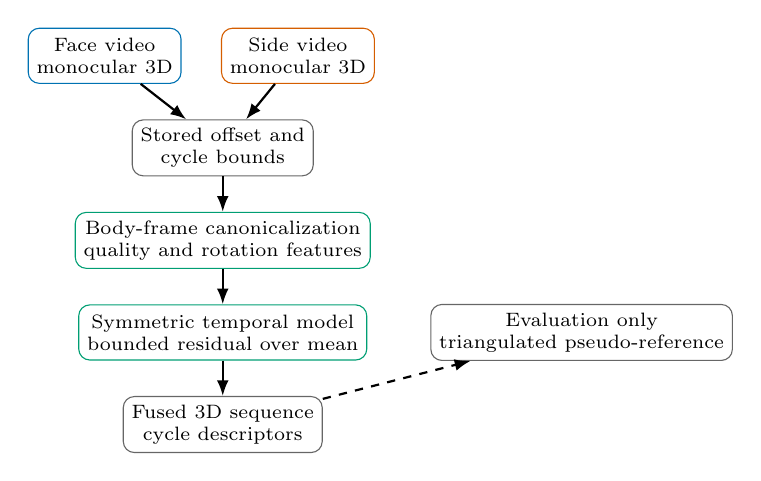
\begin{tikzpicture}[
 node distance=4.5mm and 5mm,
 box/.style={draw,rounded corners,align=center,font=\scriptsize,
   minimum height=7mm,inner sep=3pt},
 arr/.style={-{Latex[length=2mm]},thick}
]
\node[box,draw=viewblue] (face) {Face video\\monocular 3D};
\node[box,draw=vieworange,right=of face] (side) {Side video\\monocular 3D};
\node[box,draw=neutralgray,below=of face,xshift=15mm] (align)
 {Stored offset and\\cycle bounds};
\node[box,draw=fusiongreen,below=of align] (canon)
 {Body-frame canonicalization\\quality and rotation features};
\node[box,draw=fusiongreen,below=of canon] (model)
 {Symmetric temporal model\\bounded residual over mean};
\node[box,draw=neutralgray,below=of model] (output)
 {Fused 3D sequence\\cycle descriptors};
\node[box,draw=neutralgray,right=8mm of model] (eval)
 {Evaluation only\\triangulated pseudo-reference};
\draw[arr] (face) -- (align);
\draw[arr] (side) -- (align);
\draw[arr] (align) -- (canon);
\draw[arr] (canon) -- (model);
\draw[arr] (model) -- (output);
\draw[arr,dashed] (output) -- (eval);
\end{tikzpicture}
\caption{Applied workflow and supervision boundary. Triangulated 3D is
resolved only by the evaluation layer and cannot influence model training or
selection.}
\label{fig:workflow}
\end{figure}

\subsection{Self-supervision and training}

Clean cross-view observations form pseudo-targets only where evidence is
usable: closely agreeing points are quality-weighted, one clearly higher-quality
view is selected, and single-view observations are retained when the other view
is missing. Large unexplained disagreements are excluded. Seven reproducible
corruptions---joint dropout, block dropout, impulse noise, random-walk drift,
upper-body rotation bias, frozen segments and integer frame shifts---are
applied without overwriting the clean streams.

The complete model minimizes nine masked losses: corruption recovery,
high-consensus identity, axial-angle agreement, full relative-rotation
agreement, bone-length consistency, temporal bone rigidity, adaptive
acceleration agreement, minimal residual magnitude and complete-cycle axial
range. The complete-cycle term is evaluated on unpadded cycles, whereas other
terms use 128-frame windows. The model has 128 hidden channels and was optimized
with Adam for 100 epochs at learning rate $10^{-3}$ and batch size 32.
Checkpoint selection averaged fixed-corruption recovery, bone variation,
rotation consistency, identity and cycle-range scores; none used the
triangulated pseudo-reference.

\subsection{Evaluation hierarchy}

The fixed person split contained 96 training, 27 validation and 14 held-out
test participants. The 14-person set was the primary learned comparison.
Person-level mean per-joint position error was calculated after one static
sequence-level similarity transform and hip centring against the triangulated
pseudo-reference. Each comparison was paired against the complete model on the
same participants using a person-bootstrap 95\% confidence interval and a
two-sided Wilcoxon signed-rank test; Holm correction covered the nine planned
comparisons. Results use one training seed and therefore do not quantify
optimization variance.

A deterministic analysis over all 137 participants first isolated the effect of
coordinate representation by comparing world-coordinate, root-aligned,
similarity-aligned and body-frame fusion variants. The held-out learned
comparison then tested whether residual learning added evidence beyond the
canonical deterministic means. One legacy row whose joint weights were fitted
to the evaluation pseudo-reference was retained only as a leakage diagnostic
and was excluded from recommendations.

Limited external testing used 199 rendered samples from three sequences, one
Unity avatar/environment and a fixed two-camera configuration. Sixteen mapped
joints were evaluated against native Unity 3D after sequence-level similarity
alignment. The private model was applied zero-shot. Calibrated triangulation
used 2D observations and exact Unity cameras, so it is reported as a different
input regime rather than a directly matched fusion baseline.

\subsection{Downstream representation-sensitivity case study}

Ten cohort-stratified outer folds separated people, not cycles, so every
participant received an out-of-fold prediction. The resulting 928 eligible
cycles comprised 539 elderly-labeled and 389 student-labeled cycles. Each cycle
was direction-aligned and resampled to 101 phase points. Eight prespecified
descriptors covered axial rotation range, 95th-percentile angular speed,
peak-rotation phase, 95th-percentile trunk tilt, 95th-percentile wrist wrapping,
cycle duration, log dimensionless angular jerk and leave-one-cycle-out
whole-body repeatability.

For each descriptor, a cycle-level mixed model included cohort, normalized
cycle position, their interaction and outer-fold fixed effects. Cycle position
was centred at 0.5; therefore, the cohort coefficient estimates the
elderly-minus-student contrast at the mid-repetition reference. Participant
random intercepts and, when nonsingular, random cycle-position slopes accounted
for repeated cycles. Holm correction was applied separately to the eight
cohort coefficients and eight interactions. Within-person dispersion was the
participant-level median absolute deviation (MAD); groups were compared with
10,000 participant-label permutations, participant-bootstrap confidence
intervals and a separate eight-outcome Holm family. Pose-source sensitivity
repeated the centred model using face-only, side-only and deterministic
body-frame features.

\section{Results}\label{sec:results}

\subsection{Coordinate-system effect and held-out learned comparison}

Across all 137 participants, deterministic body-frame averaging had mean
pseudo-reference error 0.0640 repository units, compared with 0.1221 for
world-coordinate averaging, a 47.54\% reduction against this deliberately
uncorrected baseline. More informative leakage-free aligned variants occupied
a narrow range from 0.0640 to 0.0663 with overlapping confidence intervals.
The evidence therefore supports coordinate normalization, rather than a
particular weighting rule or learned residual, as the main source of in-domain
improvement.

\begin{table}[t]
\caption{Primary comparison on 14 held-out participants. Error is
person-level mean $\pm$ standard deviation after one sequence-level similarity
alignment to the same-video triangulated pseudo-reference. Differences are
method minus the complete model (A6); $p$ values are Holm-adjusted paired
Wilcoxon tests.}
\label{tab:heldout}
\centering
\scriptsize
\begin{tabular}{clccc}
\toprule
ID & Method & Error (mm) & Difference [95\% CI] & $p_{\rm Holm}$\\
\midrule
A0 & Face only & $77.92\pm12.52$ & $+17.14$ [13.69, 21.34] & 0.0011\\
A1 & Side only & $75.84\pm13.93$ & $+15.07$ [10.23, 19.48] & 0.0018\\
A2 & Arithmetic mean & $60.85\pm8.98$ & $+0.07$ [$-0.50$, 0.59] & 1.0000\\
A3 & Quality mean & $61.03\pm8.84$ & $+0.26$ [0.17, 0.35] & 0.0011\\
A4 & Spatial objectives & $62.81\pm8.86$ & $+2.04$ [1.71, 2.36] & 0.0011\\
A5 & Rotation/temporal & $60.80\pm8.96$ & $+0.02$ [$-0.38$, 0.43] & 1.0000\\
A6 & Complete model & $\mathbf{60.78\pm8.72}$ & --- & ---\\
\bottomrule
\end{tabular}
\end{table}

Table~\ref{tab:heldout} shows that A6 was statistically indistinguishable from
arithmetic averaging and A5. Its complete-cycle range and peak-angular-speed
retention relative to the deterministic quality mean were both 1.000, but
these ratios assess departure from the base rather than physical validity.
All canonical averaging and learned outputs were view-order invariant to the
reported precision. Validation-only corruption diagnostics did not establish a
general robustness advantage for A6: its output moved more than the
deterministic quality mean under joint and temporal-block dropout. Freer post
hoc residual variants increased error to 92.02--94.11~mm and are reported in
the Online Resource. A6 is consequently retained as the prespecified complete
test of the declared constraints, not as a demonstrated accuracy or robustness
winner.

\subsection{External native-3D test}

\begin{table}[t]
\caption{Limited external evaluation against Unity native 3D. Direct-3D and
calibrated-2D rows use different input information.}
\label{tab:unity}
\centering
\small
\begin{tabular}{llrr}
\toprule
Input & Method & Error (mm) & Angle MAE ($^\circ$)\\
\midrule
Uncalibrated 3D & World average & 166.537 & 47.497\\
Uncalibrated 3D & A6, zero-shot & 178.506 & 45.983\\
Calibrated 2D & Triangulation & 30.259 & 15.198\\
\bottomrule
\end{tabular}
\end{table}

The external result changed the interpretation (Table~\ref{tab:unity}). A6 did
not improve zero-shot positional transfer relative to direct 3D averaging.
Calibrated 2D triangulation was substantially more accurate, but used camera
geometry and evidence unavailable to the post-estimation method.

\subsection{Representation sensitivity in the repeated-cycle case study}

All eight mixed models converged. At mid-repetition, the elderly-labeled cohort
had a 0.3006 higher log angular-speed coefficient (95\% confidence interval
0.1136--0.4876, $p_{\rm Holm}=0.0114$), corresponding to a ratio of 1.351, and
a 0.4233 higher log dimensionless-jerk coefficient (0.2336--0.6130,
$p_{\rm Holm}=0.000098$). The other six corrected cohort contrasts were not
significant. No cohort-by-cycle-position interaction survived correction;
there was therefore no evidence of different monotonic first-to-last
repetition trends. Within-person jerk MAD was 0.0377 higher in the
elderly-labeled cohort (bootstrap 95\% confidence interval 0.0135--0.0735,
$p_{\rm Holm}=0.0208$); no other within-person dispersion contrast survived.

\begin{table}[t]
\caption{Sensitivity of significant A6 cohort coefficients to pose source.
Values are elderly-minus-student coefficients from the same centred mixed
model; $p$ values are Holm-adjusted within each source.}
\label{tab:sensitivity}
\centering
\scriptsize
\begin{tabular}{lrrrr}
\toprule
Outcome & OOF A6 & Face & Side & Body-frame mean\\
\midrule
Log angular speed & 0.3006 & $-0.0111$ & 0.0843 & 0.0891\\
$p_{\rm Holm}$ & 0.0114 & 1.0000 & 0.0337 & 0.0323\\
Log dimensionless jerk & 0.4233 & 0.0452 & 0.0646 & 0.0657\\
$p_{\rm Holm}$ & 0.0001 & 1.0000 & 0.2475 & 0.2324\\
\bottomrule
\end{tabular}
\end{table}

Changing the pose source materially reduced the cohort coefficients
(Table~\ref{tab:sensitivity}), especially for jerk. Separate
participant-median permutation tests were also non-significant after correction
for A6 angular speed and jerk. The stable finding from this case study is
therefore the sensitivity of downstream inference to pose representation, not
a representation-independent difference between the two labeled cohorts.

\begin{figure}[t]
\centering
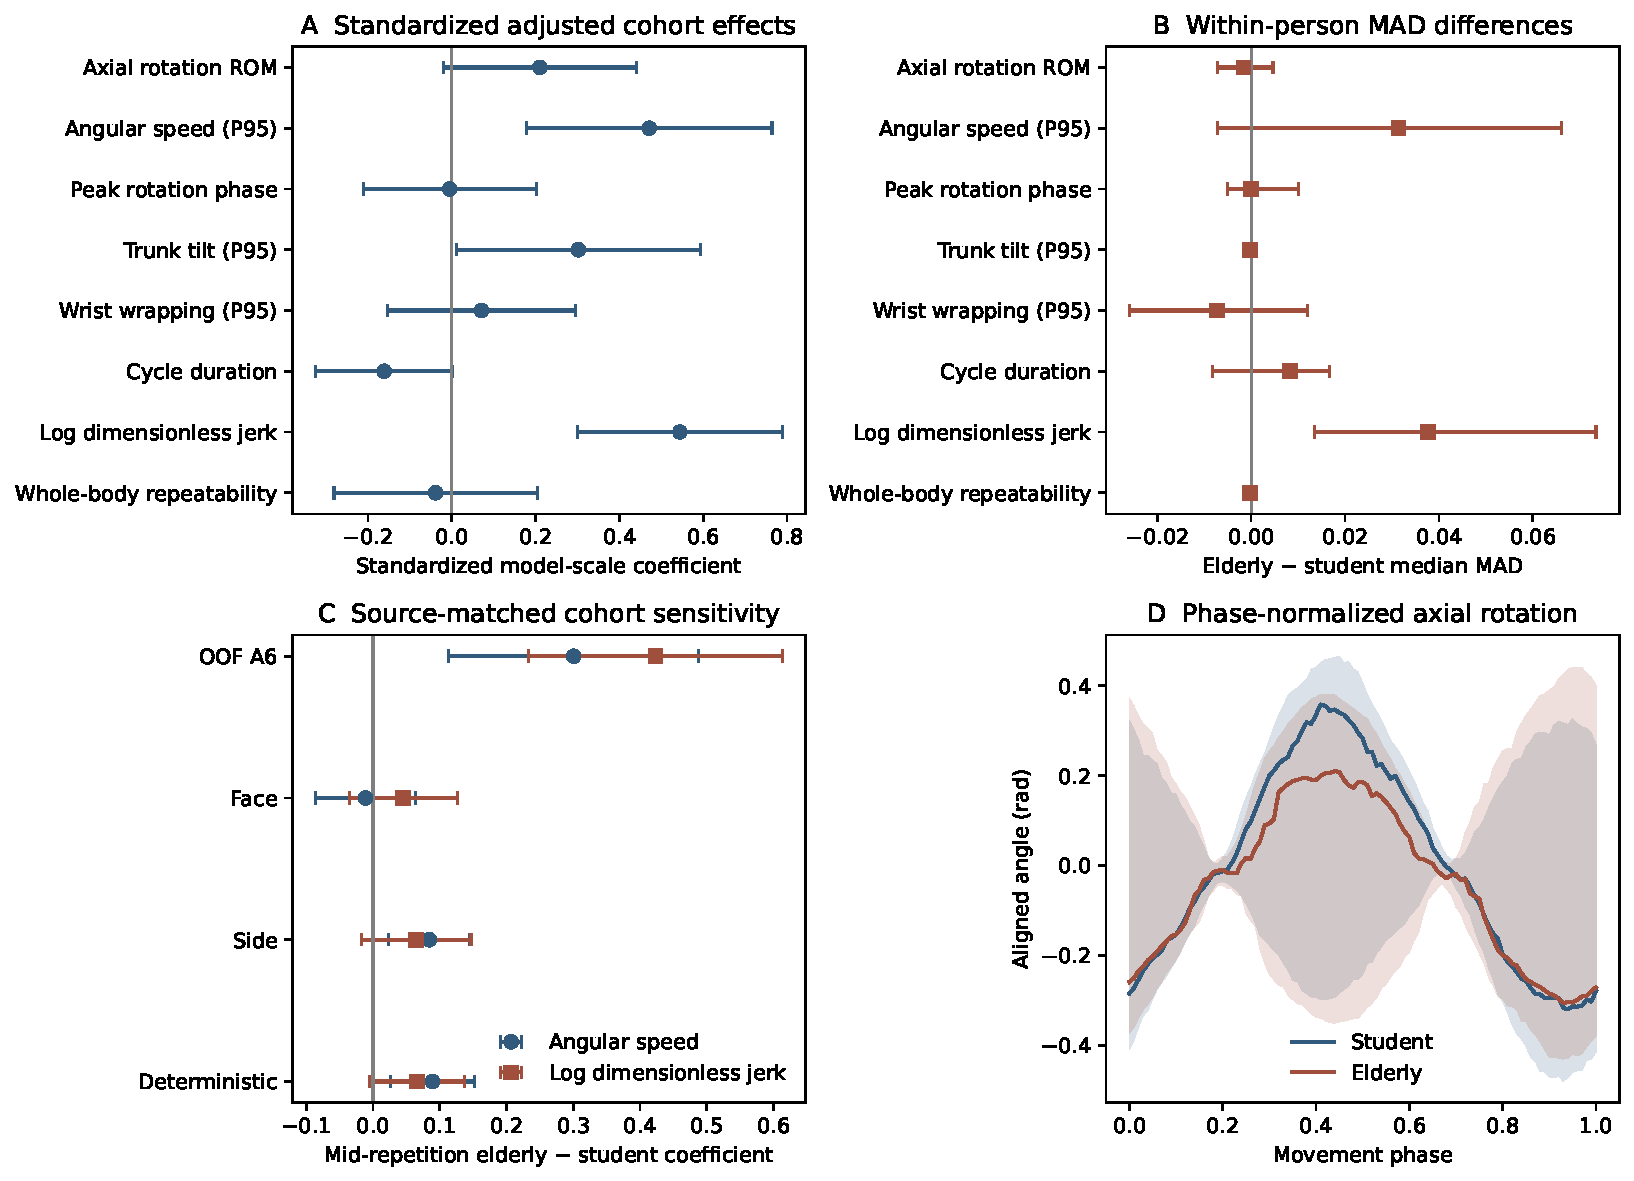
\includegraphics[width=\linewidth]{cohort_cycle_analysis.pdf}
\caption{Person-disjoint repeated-cycle analysis. (a) Standardized
mid-repetition cohort effects. (b) Differences in participant-level
within-person MAD. (c) Pose-source sensitivity for angular speed and
dimensionless jerk. Error bars are 95\% confidence intervals. (d)
Participant-median phase-normalized axial rotation with interquartile bands.}
\label{fig:cohort}
\end{figure}

\section{Discussion}\label{sec:discussion}

The most robust engineering result is the effect of the coordinate system.
Mapping both monocular streams into a pelvis-centred body frame nearly halved
their disagreement with the same-video pseudo-reference compared with
world-coordinate averaging. Once this mismatch was removed, deterministic and
learned methods occupied a narrow range. The held-out comparison provides no
evidence that the complete network improves positional accuracy over arithmetic
averaging or A5. This is evidence for coordinate harmonization, not learned
fusion superiority. A6 instead serves as the prespecified complete test of
explicit requirements: view-order invariance, bounded correction, missing-view
fallback and complete-cycle rotation constraints.

This distinction matters when an applied system is selected. If the goal is a
simple fused sequence and compute or training data are limited, deterministic
body-frame averaging is the better-supported default. The learned model is
justified when its explicit audit trail and constrained motion representation
are required, but the current results do not justify extra complexity on
position error or corruption stability. Reference-relative range and
angular-speed retention also cannot establish biomechanical validity, because
their denominator is the deterministic base rather than independent motion
capture.

Unity exposes a second boundary. A6 transferred worse than direct 3D averaging
for position, whereas calibrated triangulation from 2D evidence was far better.
Projection geometry retains information that cannot reliably be recovered
after two independent monocular 3D predictions have been made. In a prospective
capture where camera calibration is feasible, calibrated reconstruction should
therefore be preferred. Post-estimation fusion addresses archival or
low-infrastructure data where calibration is unavailable; it is not a
replacement for geometry.

The repeated-cycle experiment primarily demonstrates the risk of
representation-dependent downstream inference. Person-disjoint prediction
avoids evaluating a participant with a model trained on that participant, and
mixed models retain cycle-level information while accounting for repeated
observations. A6 produced cohort contrasts in angular speed and jerk and
greater within-person jerk dispersion, but no group-specific repetition trend.
The same models applied to other pose streams produced much smaller effects,
and participant-median tests changed the inference. The signals may combine
true movement differences, cohort composition, monocular estimation error and
learned representation effects. They must not be interpreted as ageing effects,
normative values, impairment markers or clinical findings.

The private pseudo-reference shares upstream 2D evidence with the candidate
poses and is scored after sequence-level similarity alignment. Its errors can
therefore be correlated with candidate errors, and the reported value is
agreement with a construction rather than absolute accuracy. The primary
learned test includes only 14 participants and one training seed. The Unity
test contains one avatar/environment and fixed cameras. The cohort data lack
individual demographic, health and training covariates. Finally, a single
global time offset cannot model drift, dropped frames or rolling shutter, and
the study covers one movement family and one face/side arrangement.

Future work should validate the representation against synchronized independent
capture and across diverse people, cameras and movements. Public datasets such
as Human3.6M, MPI-INF-3DHP and TotalCapture provide complementary settings
\cite{Ionescu2014Human36M,Mehta2017MPIINF3DHP,Trumble2017TotalCapture}.
For sports deployment, comparisons should include calibrated systems such as
OpenCap, whose camera calibration, musculoskeletal modelling and laboratory
validation support a different level of interpretation \cite{Uhlrich2023OpenCap}.
Repeated training seeds, local temporal alignment and measured participant
covariates are also required before the cohort analysis can progress beyond
hypothesis generation.

\section{Conclusions}\label{sec:conclusion}

Calibration-free post-estimation fusion can provide a transparent sequence
representation when only aligned monocular 3D pose streams remain available.
Pelvis-centred canonicalization provided the clearest in-domain improvement;
the complete self-supervised model matched but did not surpass strong held-out
baselines, showed no general corruption-stability advantage and did not improve
zero-shot external position accuracy. The repeated-cycle case study further
showed that between-cohort and within-person inferences changed with the pose
source. The workflow is therefore best treated as an exploratory,
low-infrastructure representation layer. Absolute biomechanical, causal or
clinical interpretation requires calibrated or independent reference capture
and richer participant information.

\bibliography{references}

\section*{Statements and Declarations}

\subsection*{Funding}
This research did not receive any specific grant from funding agencies in the
public, commercial or not-for-profit sectors.

\subsection*{Competing interests}
The author declares no competing interests.

\subsection*{Author contributions}
Kaixu Chen: conceptualization, methodology, software, validation, formal
analysis, investigation, data curation, visualization, writing---original
draft, and writing---review and editing.

\subsection*{Data availability}
The raw videos contain identifiable participant information and are not
publicly available. Code and derived anonymized keypoint data have not yet been
deposited in a public repository. Release or controlled-access conditions will
be determined after institutional ethics, participant-consent and privacy
review. Numerical results are retained in archived experiment artifacts.

\subsection*{Ethics approval and consent to participate}
\textbf{Author verification required before submission:} insert the confirmed
institutional ethics approval or exemption identifier and the participant
consent statement. No ethics status is inferred from the software repository.

\subsection*{Use of generative artificial intelligence}
During manuscript preparation, the author used OpenAI Codex for organization,
language editing, LaTeX preparation and code-assisted consistency checks. The
author reviewed and edited the resulting material and takes full responsibility
for the publication.

\subsection*{Acknowledgements}
No additional acknowledgements are declared in this draft.

\end{document}
